\documentclass[aspectratio=169,11pt]{beamer}
% Shared preamble for the CogLean decks.
% Build the slides alone, or with speaker notes (see the Makefile):
%   pdflatex deck.tex                                   -> slides
%   pdflatex -jobname=deck-notes "\def\withnotes{}\input{deck.tex}"  -> slides + notes
\usetheme{default}
\usecolortheme{seahorse}
\setbeamertemplate{navigation symbols}{}
\setbeamertemplate{footline}[frame number]
\setbeamerfont{note page}{size=\small}
\setbeamercolor{note page}{bg=white}
\ifdefined\withnotes
  \setbeameroption{show notes}
\fi
\usepackage[T1]{fontenc}
\usepackage{lmodern}
\usepackage{booktabs}
\usepackage{amsmath,amssymb}
\usepackage{tikz}
\usetikzlibrary{positioning,arrows.meta,shapes.misc}
\tikzset{
  box/.style={draw, rounded corners, align=center, minimum height=8mm, inner sep=4pt, fill=blue!6},
  arr/.style={-{Stealth[length=2mm]}, thick}
}
\newcommand{\code}[1]{\texttt{#1}}
\newcommand{\has}{\textbf{has}}
\newcommand{\lacks}{\textcolor{red!70!black}{lacks}}
\newcommand{\never}{\textcolor{red!70!black}{\textbf{never}}}
\newcommand{\canhold}{can hold}

% Lean source in slides: fvextra Verbatim, with the Unicode Lean uses mapped
% to math symbols (pdflatex).
\usepackage{fvextra}
\fvset{fontsize=\scriptsize, frame=single, framesep=2mm, rulecolor=\color{gray!50},
  breaklines=true, breakanywhere=false}
\DeclareUnicodeCharacter{2192}{\ensuremath{\to}}
\DeclareUnicodeCharacter{2190}{\ensuremath{\leftarrow}}
\DeclareUnicodeCharacter{2194}{\ensuremath{\leftrightarrow}}
\DeclareUnicodeCharacter{2200}{\ensuremath{\forall}}
\DeclareUnicodeCharacter{2203}{\ensuremath{\exists}}
\DeclareUnicodeCharacter{27E8}{\ensuremath{\langle}}
\DeclareUnicodeCharacter{27E9}{\ensuremath{\rangle}}
\DeclareUnicodeCharacter{2260}{\ensuremath{\neq}}
\DeclareUnicodeCharacter{2227}{\ensuremath{\wedge}}
\DeclareUnicodeCharacter{2228}{\ensuremath{\vee}}
\DeclareUnicodeCharacter{00AC}{\ensuremath{\neg}}
\DeclareUnicodeCharacter{2264}{\ensuremath{\le}}
\DeclareUnicodeCharacter{2208}{\ensuremath{\in}}
\DeclareUnicodeCharacter{2209}{\ensuremath{\notin}}
\DeclareUnicodeCharacter{00D7}{\ensuremath{\times}}
\DeclareUnicodeCharacter{03B1}{\ensuremath{\alpha}}
\DeclareUnicodeCharacter{03B2}{\ensuremath{\beta}}
\DeclareUnicodeCharacter{03BC}{\ensuremath{\mu}}
\DeclareUnicodeCharacter{03B8}{\ensuremath{\theta}}
\DeclareUnicodeCharacter{2218}{\ensuremath{\circ}}
\DeclareUnicodeCharacter{25B8}{\ensuremath{\blacktriangleright}}
\DeclareUnicodeCharacter{00B7}{\ensuremath{\cdot}}
\DeclareUnicodeCharacter{2026}{\ldots}

\usepackage{array}
\tikzset{src/.style={rounded corners=8pt, draw=none, align=center, inner sep=6pt,
    text width=#1, font=\small\bfseries, execute at begin node={\hyphenpenalty=10000\exhyphenpenalty=10000}},
  src/.default=3.5cm,
  to/.style={-{Stealth[length=2.2mm]}, thick, black!80}}

\title{CogLean}
\subtitle{Towards a Cumulative, Machine-Checked Theory of Cognition}
\author{Jeff Shrager}
\date{October 2026\\[2mm]\small\textcolor{red!70!black}{\textbf{Draft for Comment}}}

\begin{document}

% Head slides: the word, then where it came from.
\begin{frame}[plain]
  \begin{tikzpicture}[remember picture,overlay]
    \node at (current page.center) {\fontsize{54}{60}\selectfont\bfseries\itshape Epoofany};
  \end{tikzpicture}
\end{frame}
\note{
Epoofany.
}

\begin{frame}[plain]
  \begin{tikzpicture}[remember picture,overlay]
    \node[draw=orange!80!black, very thick, rounded corners=10pt, fill=orange!8,
          align=center, inner sep=8pt] (c) at (current page.center)
      {{\fontsize{40}{46}\selectfont\bfseries CogLean}\\[-2pt]
       \rule{4.2cm}{0.6pt}\\[2pt]
       {\itshape Don't just run models,}\\ {\itshape reason about them.}};
    \begin{scope}[shift={(current page.center)}]
      \node[src=3.7cm, fill=blue!12] (tl) at (-5.2, 2.85)
        {Reanimation of Simon \& Newell's early AIs\\ {\mdseries\itshape (esp.\ LT and EPAM)}};
      \node[src=3.3cm, fill=violet!12] (tc) at (0, 3.1)
        {Discussion with Pete and Chris on models of scientific reasoning};
      \node[src=3.6cm, fill=violet!18] (tr) at (5.2, 2.85)
        {NSS's theory of computer programs as cognitive models};
      \node[src=3.4cm, fill=green!12, align=left] (ml) at (-5.9, 0)
        {Training with Simon and Klahr during the {\mdseries\itshape Scientific Cognition} period};
      \node[src=3.4cm, fill=yellow!18] (mr) at (5.9, 0)
        {Work with Siegler on the DOA model};
      \node[src=3.4cm, fill=red!12] (bl) at (-5.2, -2.9)
        {Work with Anderson on ACT};
      \node[src=3.4cm, fill=blue!12] (br) at (5.2, -2.9)
        {The Lean-driven mathpocalypse};
    \end{scope}
    \draw[to] ([yshift=-2mm]tl.east) -- ([xshift=4mm]c.north west);
    \draw[to] (tc.south) -- (c.north);
    \draw[to] ([yshift=-2mm]tr.west) -- ([xshift=-4mm]c.north east);
    \draw[to] (ml.east) -- (c.west);
    \draw[to] (mr.west) -- (c.east);
    \draw[to] ([yshift=2mm]bl.east) -- ([xshift=4mm]c.south west);
    \draw[to] ([yshift=2mm]br.west) -- ([xshift=-4mm]c.south east);
  \end{tikzpicture}
\end{frame}
\note{
Where CogLean came from.
}

\begin{frame}
  \titlepage
\end{frame}
\note{
This talk goes with the paper of the same name, which is a draft for comment. It hasn't been carefully checked yet: think of it as an over-starched blog post, and constructive feedback is welcome. The paper introduces CogLean, a library of cognitive theory in the Lean proof assistant, and argues for a way of doing theoretical cognitive science: theories stated once, their consequences proved, and independently developed theories composed so that new results follow from old ones. I'm going to tell it through a hypothetical modeler, Chris, who uses the library to answer two questions about children's arithmetic: one forward, from a phenomenon to a theorem, and one backward, from a proposed regularity to what a theory must be like to produce it. The central example is multi-digit addition, but I want to be clear from the start that it is a demonstration, not a new theory of arithmetic.
}

\begin{frame}{The problem: making theory cumulative}
  \begin{itemize}
    \item Newell (1973): twenty questions with nature, answers never assembled; Newell (1990): unified theories.
    \item Cognitive architectures (Soar, ACT-R; now the Common Model) have spent decades on this: \textbf{shared mechanisms}, so models of different tasks reuse and integrate theoretical commitments.
    \item What they accumulate is mainly \textbf{models}: what a model predicts is established by running it, one setting at a time, and a result for one model is rarely reusable \emph{as a result} by another.
    \item CogLean, \textbf{complementary}: accumulate machine-checked \textbf{theorems} about mechanisms, reusable deductively, and stated across architectural commitments.
  \end{itemize}
  \bigskip
  \emph{Can independently developed theories, in a common formal library, be composed to derive meaningful consequences we'd otherwise need a new model to find?}
\end{frame}
\note{
The problem is an old one, and the people who have done the most about it are the architecture builders. Newell complained in 1973 that we play twenty questions with nature and never assemble the answers, and his answer was unified theories of cognition. Soar and ACT-R, and now the Common Model of Cognition, are decades of work by Newell, Anderson, Laird, Rosenbloom and many others on exactly this: shared mechanisms and constraints, so that a model of a new task reuses the architecture's theory of memory, learning and control, and models of different tasks can be integrated. CogLean is not the first effort in this direction, and it isn't a competitor. What architectures accumulate, though, is mainly models. What a model predicts is established by running it, at one setting at a time, and a result established for one model is rarely available as a result to another. CogLean pursues a complementary goal: accumulating machine-checked theorems about cognitive mechanisms, which can be reused deductively, and stated independently of any one architecture's commitments, so they can cover classes of mechanisms. An architecture could, in principle, carry such results itself. The question for this talk is whether a common formal library can change that: whether theories in such a library can be composed to give meaningful consequences that we would otherwise need a whole new model to find.
}

\begin{frame}{Prior formal approaches to cognitive theory}
  \scriptsize
  \begin{tabular}{>{\raggedright\arraybackslash}p{0.34\linewidth}>{\raggedright\arraybackslash}p{0.19\linewidth}>{\raggedright\arraybackslash}p{0.36\linewidth}}
    \toprule
    Work & Formalism & What it establishes\\
    \midrule
    Soar specified in Z (Milnes et al.\ 1992) & Z notation & a complete, low-level, non-executable specification of one architecture\\
    Sceptic (Cooper, Fox, Farringdon \& Shallice 1996) & executable specification language & models (Soar among them) stated in a language designed for cognitive models\\
    Reconstructing ACT-R (Stewart \& West 2007) & Python reimplementation & core commitments separated from implementation; alternative components\\
    ACT-R operational semantics (Gall \& Fr\"uhwirth 2018) & abstract semantics; CHR & a translation proved sound and complete; confluence tests\\
    ACT-R as timed automata (Langenfeld et al.\ 2019, 2021) & timed automata & exhaustive defect analysis of models; the semantics proved correct\\
    A common formal ground for architectures (Ragni et al.\ 2018) & formal framework & ACT-R and Soar embedded for comparison\\
    Soar to PRISM (Ganeriwala et al.\ 2026) & Markov chains, PRISM & probabilistic model checking of stochastic models\\
    Verbal theories as logic programs; as automata (Rohner \& Kjellerstrand 2021; Finkel et al.\ 2025) & Prolog; automata & what a verbal theory's premises entail\\
    Critical tests from core assumptions (Fisher et al.\ 2025) & proofs in prose over model classes & which processing structures ACT-R's core rules out\\
    \bottomrule
  \end{tabular}
\end{frame}
\note{
CogLean is far from the first formal treatment of cognitive theory, and it's worth seeing what came before. In 1992 Milnes and colleagues specified Soar in the Z notation: complete, but low-level and not executable. Cooper, Fox, Farringdon and Shallice argued in 1996 for languages designed for specifying cognitive models, and built one, Sceptic. Stewart and West rebuilt ACT-R to separate its core commitments from its implementation. For ACT-R there's a formal operational semantics with a translation proved sound and complete, and a line of work translating ACT-R models into timed automata for exhaustive defect checking. Ragni and colleagues proposed a common formal ground into which ACT-R and Soar can be embedded. Most recently, Soar models have been compiled for the PRISM probabilistic model checker. Outside architectures, verbal theories have been formalized as logic programs and as automata, and Fisher and colleagues derived critical tests of ACT-R from its core assumptions. Almost all of this work formalizes one architecture or one model at a time, and establishes properties of that system. That's the contrast I'll come back to.
}

\begin{frame}{The analogy: Mathlib}
  \begin{itemize}
    \item Mathlib, the community library of formalized mathematics in Lean, proposes no new mathematics.
    \item It is a \textbf{shared environment}: definitions made once, every result machine-checked, later work citing earlier results.
    \item A theorem about groups, once proved, is available to everyone who uses groups.
  \end{itemize}
  \bigskip
  CogLean asks whether cognitive theory can be organized the same way.\\
  It is not a new theory of cognition, nor a new modeling language.\\
  And it is nowhere near Mathlib's scale: a first demonstration.
\end{frame}
\note{
Mathematics faced a version of this problem and has made real progress on it. Mathlib, the community library for the Lean proof assistant, doesn't propose new mathematics. It's a shared environment: definitions are made once, every result is checked by machine, and later work builds on earlier results by citing them. A theorem about groups, once proved, is available to everyone who works with groups. CogLean asks whether cognitive theory can be organized the same way. It is not a new theory of cognition, and it's not a new modelling language either. And it's nowhere near Mathlib's scale; this is a first demonstration that the approach can work.
}

\begin{frame}{CogLean's layers}
  \begin{center}
  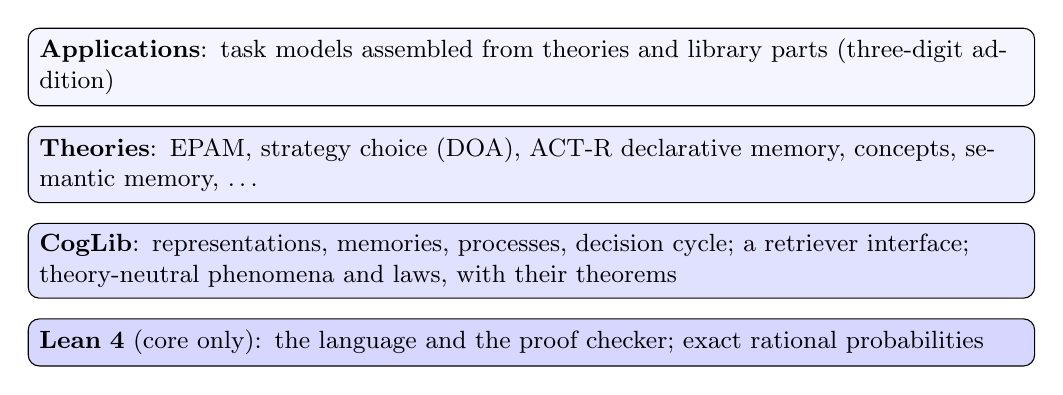
\begin{tikzpicture}[font=\small, node distance=2.5mm,
    layer/.style={draw, rounded corners, text width=12.5cm, align=left, inner sep=4pt}]
    \node[layer, fill=blue!4] (app) {\textbf{Applications}: task models assembled from theories and library parts (three-digit addition)};
    \node[layer, fill=blue!8, below=of app] (th) {\textbf{Theories}: EPAM, strategy choice (DOA), ACT-R declarative memory, concepts, semantic memory, \dots};
    \node[layer, fill=blue!12, below=of th] (lib) {\textbf{CogLib}: representations, memories, processes, decision cycle; a retriever interface; theory-neutral phenomena and laws, with their theorems};
    \node[layer, fill=blue!16, below=of lib] (lean) {\textbf{Lean 4} (core only): the language and the proof checker; exact rational probabilities};
  \end{tikzpicture}
  \end{center}
  Each layer imports only those below it, and inherits their theorems.
\end{frame}
\note{
CogLean has four layers. At the bottom is Lean, core only, with exact rational probabilities. Above it is CogLib, the general library: representations such as feature codes and distributions; memory structures such as discrimination nets and an activation memory; processes such as sampled retrieval and a decision cycle with impasses; an interface that any memory can implement; and theory-neutral statements of phenomena and laws, with theorems about them. Above that are the theories, each stated as choices of library mechanisms. And at the top are applications, models of particular tasks assembled from theories and library parts. Each layer imports only those below it, and inherits their theorems.
}

\begin{frame}{Four kinds of object, kept apart}
  \begin{enumerate}
    \item \textbf{Mechanisms} and their postulates: definitions (how a net sorts a code; how retrieval samples).
    \item \textbf{Phenomena}: predicates, stated without any mechanism. A predicate asserts nothing; it is a target.
    \item \textbf{Theorems}: a mechanism produces behavior satisfying a predicate.
    \item \textbf{Conditions}: situational (``$x$ is confused with $q$''), empirical premises not yet explained (``associations are sharp''), well-formedness.
  \end{enumerate}
  \bigskip
  A theorem with a phenomenon among its hypotheses is a relation between phenomena, not a prediction. The catalog flags these mechanically.
\end{frame}
\note{
Four kinds of object have to be kept apart. Mechanisms and their postulates are definitions. Phenomena are predicates, stated without reference to any mechanism; a predicate asserts nothing, it's a target. Theorems say that a mechanism produces behaviour satisfying a predicate. And conditions are the hypotheses under which a theorem holds: some situational, some empirical premises we haven't explained yet, some just well-formedness. One rule follows: a theorem with a phenomenon among its hypotheses is a relation between phenomena, not a prediction of any model. The library's catalog flags those mechanically.
}

\begin{frame}{Meet Chris (and Robin)}
  \begin{itemize}
    \item \textbf{Chris}: a hypothetical cognitive scientist who studies how children learn arithmetic, and has built models before.
    \item The usual workflow: write a program that implements the mechanisms; run it; explain the results in a paper.
    \begin{itemize}
      \item The program specifies the mechanisms.
      \item The \emph{reasoning} about their consequences lives in Chris's head, the comments, the prose.
    \end{itemize}
    \item CogLean supports \textbf{programming} a mechanism \emph{and} \textbf{reasoning formally} about it; the reasoning is checked, kept as theorems, reused.
    \item \textbf{Robin}: Chris's chatbot research colleague. Good at brainstorming, finding library results, suggesting proofs. \emph{Not} automatically right.
  \end{itemize}
  \medskip
  \centering\small Chris poses the questions $\cdot$ Robin suggests $\cdot$ Lean checks $\cdot$ evidence decides
\end{frame}
\note{
Let me introduce Chris. Chris is a hypothetical cognitive scientist who studies how children learn arithmetic, and has built computational models before. Like most of us, Chris is used to a particular workflow: write a program that implements the proposed mechanisms, run it to see what it does, and explain the results in a paper. The program specifies the mechanisms, but the reasoning about what they imply lives in Chris's head, in the comments, or in the prose. CogLean offers another way to work. It supports programming a mechanism and also reasoning formally about it, and that reasoning is checked by the computer, kept as theorems, and reusable in other models. Chris also has a colleague, Robin, who is a chatbot. Robin is genuinely useful: for brainstorming, for finding what's already in the library, for suggesting proofs. But Robin is not automatically right, and you'll see Robin be wrong. The division of labor is: Chris poses the questions, Robin suggests, Lean checks, and evidence decides which premises describe children.
}

\begin{frame}{Chris's two questions}
  \begin{enumerate}
    \item \textbf{Forward: from an observation to a theorem.}\\
      Children sometimes confidently answer $150+100$ with $200$. Does that follow from existing mechanisms, and under what conditions?\\
      \small\textcolor{black!60}{Formalization; composition of theories and of their theorems; results for classes of memories.}
    \medskip
    \item \textbf{Backward: what must a theory be like?}\\
      Chris conjectures a regularity about practice and backup use. Which readings of the theory guarantee it, and which break it?\\
      \small\textcolor{black!60}{Discovery: an exposed ambiguity, a counterexample, a proof, and the assumption the regularity needs.}
  \end{enumerate}
  \medskip
  Then: what's under the hood, and what all this does and doesn't show.
\end{frame}
\note{
Chris has two questions, and they're the two halves of the talk. The first goes forward, from an observation to a theorem. Children sometimes confidently answer one fifty plus one hundred with two hundred. Does that follow from mechanisms we already have, and under exactly what conditions? Answering it uses formalization, composition of independently formalized theories and of their theorems, and results that hold for whole classes of memories. The second goes backward. Chris conjectures a regularity about practice and backup use, and asks what a theory has to be like to guarantee it. That one exposes an ambiguity in the theory, produces a counterexample and a proof, and isolates the assumption the regularity needs. After that I'll open the hood on the composition, and finish with what all this does and doesn't show.
}

\begin{frame}[plain]
  \centering\vfill
  {\small\textcolor{black!55}{Part 1}}\\[2mm]
  {\Large\bfseries From an observation to a theorem}\\[3mm]
  {\itshape Does confident error follow from mechanisms we already have?}
  \vfill
\end{frame}
\note{
Part one. Chris's first question, going forward: does a familiar phenomenon, confident errors, follow from mechanisms already in the library?
}

\begin{frame}{Chris's observation}
  \begin{itemize}
    \item Children sometimes \textbf{confidently} give a wrong answer, apparently retrieving it rather than calculating.
    \item A child who knows $100+100=200$ takes $150+100$ for the familiar problem, and says \textbf{200}, without hesitating.
    \item Chris's question: does this follow from recognizable properties of \emph{existing} mechanisms?
  \end{itemize}
  \medskip
  \textbf{Robin}: CogLib has a general mechanism for exactly this shape,
  \begin{center}
  recognize a stimulus $\to$ retrieve an associated response $\to$ back up if retrieval fails,
  \end{center}
  and two theories already formalized that fill it in.
\end{frame}
\note{
Here's Chris's observation. Children sometimes give a wrong answer confidently: they seem to be retrieving it, not calculating it. A child who knows one hundred plus one hundred is two hundred takes one fifty plus one hundred for the familiar problem, and says two hundred without hesitating. Chris's question is whether that follows from recognizable properties of mechanisms we already have, rather than from something invented for the purpose. Robin points out that the library has a general mechanism of exactly this shape: recognize a stimulus, retrieve a response associated with what was recognized, and fall back on a backup process if retrieval fails. And two existing theories, already formalized on their own, fill it in.
}

\begin{frame}{Two theories, formalized on their own}
  \begin{columns}[T]
    \column{0.48\linewidth}
    \textbf{EPAM} (Feigenbaum \& Simon)
    \begin{itemize}
      \item A discrimination net sorts a code to a stored image.
      \item Learning grows a test only where codes are confused.
      \item Proved for every net: recognition depends only on tested features; learning never disturbs other items.
    \end{itemize}
    \column{0.48\linewidth}
    \textbf{DOA} (Siegler \& Shrager 1984)
    \begin{itemize}
      \item Associations from problems to answers; sample, state if above a criterion; else fingers, then counting.
      \item Proved for every setting: retrieval used with probability $1-(1-R)^n$; counting errors independent of the associations.
    \end{itemize}
  \end{columns}
\end{frame}
\note{
The two theories Robin has in mind were each formalized on their own, long before Chris's question. EPAM, Feigenbaum and Simon's model, recognizes a stimulus by sorting its code down a discrimination net; learning grows a test only where two codes are confused. Proved for every net: recognition depends only on the features tested, and learning never disturbs what's already learned. And the distributions-of-associations model that Bob Siegler and I proposed in 1984: a child samples answers in proportion to strength, states one that clears a confidence criterion, and otherwise falls back on fingers and counting. Proved for every setting: retrieval is used with probability one minus one minus R to the n, and counting errors don't depend on the associations at all, which was the chapter's nonintuitive prediction.
}

\begin{frame}{The application: three-digit addition}
  \begin{center}
  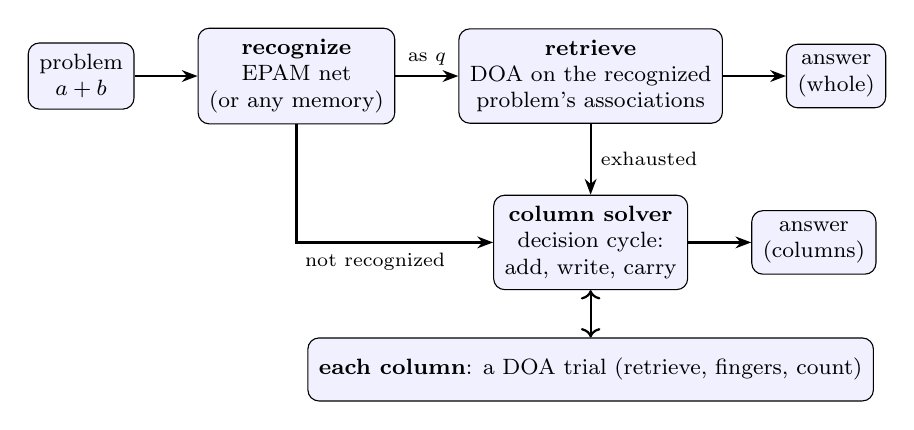
\begin{tikzpicture}[font=\footnotesize, node distance=6mm and 8mm]
    \node[box] (x) {problem\\$a+b$};
    \node[box, right=of x] (rec) {\textbf{recognize}\\EPAM net\\(or any memory)};
    \node[box, right=of rec] (ret) {\textbf{retrieve}\\DOA on the recognized\\problem's associations};
    \node[box, right=of ret] (ans) {answer\\(whole)};
    \node[box, below=9mm of ret] (sol) {\textbf{column solver}\\decision cycle:\\add, write, carry};
    \node[box, right=of sol] (ans2) {answer\\(columns)};
    \node[box, below=6mm of sol] (f) {\textbf{each column}: a DOA trial (retrieve, fingers, count)};
    \draw[arr] (x) -- (rec); \draw[arr] (rec) -- node[above, font=\scriptsize] {as $q$} (ret);
    \draw[arr] (ret) -- (ans);
    \draw[arr] (ret) -- node[right, font=\scriptsize] {exhausted} (sol);
    \draw[arr] (rec) |- node[below, pos=0.7, font=\scriptsize] {not recognized} (sol);
    \draw[arr] (sol) -- (ans2);
    \draw[arr, <->] (sol) -- (f);
  \end{tikzpicture}
  \end{center}
  \small A demonstration, not a theory of arithmetic. In Lean, the composition is three definitions.
\end{frame}
\note{
Chris composes them into a model of three-digit addition. A problem is recognized by an EPAM net, or by any memory. If it's recognized as a familiar problem q, the answer is retrieved from q's distribution of associations. If retrieval is exhausted, or nothing is recognized, a column solver takes over. It runs on the library's decision cycle, adding, writing and carrying, and each column's addition is itself a full single-digit trial from the strategy-choice model. In Lean the whole composition is three definitions. Again: arithmetic is the demonstration. It's a familiar task that needs several mechanisms, and two of the theories already existed.
}

\begin{frame}{The phenomenon, stated without a mechanism, and when it follows}
  If $q$ is recognized as itself, $x$ is confused with $q$, $q$'s associations are \textbf{sharp}, and their sums differ:
  \begin{enumerate}[(i)]
    \item whole-problem retrieval never errs on $q$;
    \item every whole-problem answer to $x$ is wrong;
    \item $x$ reaches the solver \emph{exactly as often} as $q$.
  \end{enumerate}
  \medskip
  \begin{itemize}
    \item \textbf{Neither theory alone}: in DOA, errors and backup use come from one distribution; recognition gives $x$ another problem's distribution.
    \item \textbf{Reused}: a one-line proof, from CogLib's theorem for \emph{any} task with problems, a familiar set and a backup.
    \item \textbf{Conditions}: confusion (derived for learned nets); sharpness (assumed, not yet explained); positive strengths.
  \end{itemize}
\end{frame}
\note{
Chris and Robin first state the phenomenon without mentioning EPAM or DOA: a confused problem gets wrong answers from whole-problem retrieval, but uses its backup exactly as often as the problem it's confused with. Then they look for the conditions under which it follows. Suppose a familiar problem q is recognized as itself, a stranger x is confused with it, q's associations are sharp, meaning only q's correct sum clears the criterion, and the two sums differ. Then retrieval never errs on q, every whole-problem answer to x is wrong, and x goes to the solver exactly as often as q does. Neither theory says this alone: in strategy choice, a problem's errors and its backup use come from the same distribution, so they go together. Recognition breaks the tie by handing x another problem's distribution. The proof is one line, applying a library theorem that holds for any task with problems, a familiar set and a backup. And the conditions are explicit: confusion, which is derived for learned nets; sharpness, which is assumed and not yet explained; and positive strengths.
}

\begin{frame}{In words: the theorem on the next slide}
  CogLib's \code{confident\_errors}, for \emph{any} task, memory and backup:
  \begin{itemize}
    \item \textbf{Parameters}: how problems are coded, what memory calls up (\code{retrieve}), the associations (\code{str}), the criterion and search length, and the backup.
    \item \textbf{Hypotheses}:
    \begin{itemize}
      \item strengths have positive totals; the backup is a proper distribution;
      \item $q$ calls up itself, for certain (\code{hq});
      \item $x$ calls up $q$, for certain (\code{hx}): the confusion;
      \item $q$'s associations are sharp (\code{hs}); the correct answers differ (\code{hne}).
    \end{itemize}
    \item \textbf{Conclusion}: the \emph{confusion-error pattern}, a phenomenon defined once in CogLib, apart from any mechanism: three equations, (i)--(iii) of the last slide.
    \item \textbf{Proof}: three lines, citing three earlier lemmas.
  \end{itemize}
\end{frame}
\note{
The next slide shows the actual Lean theorem, so here it is in words first. It's the library's version, which holds for any task, any memory and any backup. Its parameters are how problems are coded, what memory calls up for a code, the associations, the criterion and search length, and the backup. Its hypotheses: well-formedness of the strengths and the backup; the familiar problem calls up itself for certain; the stranger calls up the familiar problem for certain, which is the confusion; the familiar problem's associations are sharp; and the correct answers differ. The conclusion is the confusion-error pattern, which the library defines once, as a phenomenon, with no mechanism in it: the three equations from the previous slide. And the proof is three lines, each citing an earlier lemma.
}

\begin{frame}[fragile]{The theorem, in Lean}
\begin{Verbatim}[fontsize=\scriptsize, breaklines=false]
theorem confident_errors (correct : P → A) (x q : P) (hT : ∀ y, total as (str y) ≠ 0)
    (hbx : mass (backup x) = 1) (hbq : mass (backup q) = 1)
    (hq : retrieve (code q) = pure (some (code q)))
    (hx : retrieve (code x) = pure (some (code q)))
    (hs : Sharp str cc (code q) (correct q)) (hne : correct x ≠ correct q) :
    Phenomena.ConfusionErrorPattern (recognizeRetrieve code retrieve str as cc n backup)
      (wholeWrong correct) isWhole isBackup x q := by
  refine ⟨confusion_gives_neighbours_answer code retrieve str as cc n backup
      correct q q (hT _) hq hs,
    wrong_eq_whole_of_sharp code retrieve str as cc n backup
      correct x _ _ (hT _) hx hs hne, ?_⟩
  rw [backup_prob_certain code retrieve str as cc n backup x _ hx hbx hT,
    backup_prob_certain code retrieve str as cc n backup q _ hq hbq hT]

def ConfusionErrorPattern (trial : P → Dist O) (wholeWrong : P → O → Bool)
    (isWhole isBackup : O → Bool) (x q : P) : Prop :=
  prob (trial q) (wholeWrong q) = 0 ∧
    prob (trial x) (wholeWrong x) = prob (trial x) isWhole ∧
    prob (trial x) isBackup = prob (trial q) isBackup
\end{Verbatim}
  \footnotesize Verbatim from CogLib (\code{Process/RecognizeRetrieve}, \code{Phenomena/ConfusionErrors}). The multi-digit version is a one-line instance.
\end{frame}
\note{
Here's the theorem itself, verbatim from the library. The first five lines are the hypotheses, each named: h T, the two backup hypotheses, h q, h x, h s and h n e. Then the conclusion: the trial has the confusion-error pattern. Then the proof. At the bottom is that pattern's definition, three equations joined by and, about observable outcomes only. The first clause is the lemma that a problem recognized as a sharp q gets only q's answer; the second is the lemma that all its whole-problem answers are then wrong; and the third rewrites both backup probabilities with the lemma that backup use after certain recognition depends only on what's recognized. Nothing in the statement mentions arithmetic, EPAM or ACT-R. The multi-digit model's theorem is a one-line instance of this one.
}

\begin{frame}{One clause, unpacked: the confusion}
  \begin{center}
  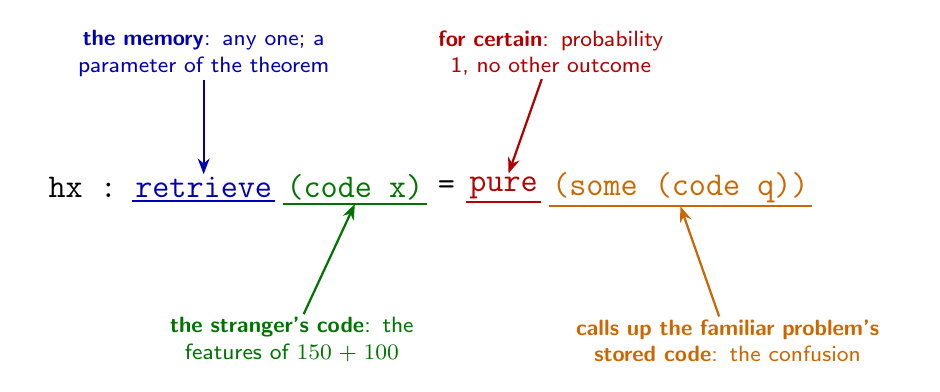
\begin{tikzpicture}[font=\ttfamily\large, inner sep=1pt, baseline]
    \node (h) {hx :};
    \node[right=1.5mm of h, text=blue!70!black] (r) {retrieve};
    \node[right=1mm of r, text=green!45!black] (c) {(code x)};
    \node[right=1mm of c] (e) {=};
    \node[right=1mm of e, text=red!70!black] (p) {pure};
    \node[right=1mm of p, text=orange!80!black] (s) {(some (code q))};
    \draw[blue!70!black, thick] (r.south west) -- (r.south east);
    \draw[green!45!black, thick] (c.south west) -- (c.south east);
    \draw[red!70!black, thick] (p.south west) -- (p.south east);
    \draw[orange!80!black, thick] (s.south west) -- (s.south east);
    \node[font=\footnotesize\sffamily, text width=4.4cm, align=center, text=blue!70!black, above=12mm of r] (ar) {\textbf{the memory}: any one; a parameter of the theorem};
    \node[font=\footnotesize\sffamily, text width=3.4cm, align=center, text=green!45!black, below=14mm of c, xshift=-8mm] (ac) {\textbf{the stranger's code}: the features of $150+100$};
    \node[font=\footnotesize\sffamily, text width=3.6cm, align=center, text=red!70!black, above=12mm of p, xshift=6mm] (ap) {\textbf{for certain}: probability 1, no other outcome};
    \node[font=\footnotesize\sffamily, text width=4.6cm, align=center, text=orange!80!black, below=14mm of s, xshift=6mm] (as) {\textbf{calls up the familiar problem's stored code}: the confusion};
    \draw[arr, blue!70!black] (ar) -- (r);
    \draw[arr, green!45!black] (ac) -- (c.south);
    \draw[arr, red!70!black] (ap) -- (p);
    \draw[arr, orange!80!black] (as) -- (s.south);
  \end{tikzpicture}
  \end{center}
  \vspace{-2mm}
  \small
  \begin{itemize}
    \item \textbf{EPAM}: holds for the net learned from $100+100$ and $100+200$ (checked); every learned net recognizes its own images.
    \item \textbf{ACT-R}: \emph{never} holds, because \code{pure} is too strong: retrieval is graded, never certain. That is why the theorem doesn't apply to it.
  \end{itemize}
\end{frame}
\note{
Let's unpack one clause, the confusion, h x. Read it left to right. Retrieve is the memory, and it's a parameter: the theorem holds for any memory you plug in. Code x is the stranger's feature code, here the features of one fifty plus one hundred. Pure means for certain: the distribution with a single outcome, at probability one. And some code q says the outcome is the familiar problem's stored code. So the clause says: this memory calls up the familiar problem, for certain, when given the stranger. For EPAM it holds: the net learned from one hundred plus one hundred and one hundred plus two hundred is checked to do exactly this. For ACT-R it never holds, and the culprit is the word pure: ACT-R's retrieval is graded and never certain. That single word is why the theorem applies to one memory and not the other.
}

\begin{frame}{Equal is not low}
  \begin{itemize}
    \item The theorem gives \emph{equal} solver use for $x$ and $q$, not \emph{low} solver use.
    \item The rate is $(1-R_q)^n$, with $R_q$ the chance one search of $q$'s associations clears the criterion.
    \item If $R_q \ge r$, the confused problem reaches the solver with probability at most $(1-r)^n$.
    \item With flat associations on $q$, the same theorem holds, and the errors are not confident.
  \end{itemize}
  \medskip
  Here $R_q = 45/46$, $n = 1$: the solver is reached $1/46$ of the time.
\end{frame}
\note{
One precision matters here. The theorem says the confused problem reaches the solver exactly as often as the familiar one. It doesn't say that's rare. The rate is one minus R q to the n, where R q is the chance that one search of q's associations clears the criterion; and if R q is at least r, solver use is at most one minus r to the n. Both are proved. So whether these errors are confident, fluent and unhesitating, is a separate, quantitative matter. With flat associations the same theorem holds, but the errors wouldn't be confident. In our setting R q is forty-five over forty-six, so the solver is reached once in forty-six.
}

\begin{frame}{Does it need EPAM? Swapping the memory}
  \small
  \begin{tabular}{lcc}
    \toprule
    & EPAM net & ACT-R memory\\
    \midrule
    $150+100$ answered 200 by retrieval & $45/46$ & $225/529 \approx .43$\\
    $150+100$: solver invoked & $1/46$ & $383/1058 \approx .36$\\
    \quad solver correct, \emph{given} invoked & $\approx .656$ & $\approx .656$\\
    \quad correct overall (invoked \emph{and} correct) & $\approx .014$ & $\approx .238$\\
    practiced $100+100$: overall errors & $\approx .0073$ & $\approx .334$\\
    \quad after also studying $100+300$ & unchanged & $\approx .616$\\
    \midrule
    memory laws (every setting) & determinacy, certainty, & none of them\\
    & stability & \\
    \bottomrule
  \end{tabular}
  \normalsize
  \medskip
  \begin{itemize}
    \item The confident-error theorem holds for \emph{any} memory with the three laws.
    \item For ACT-R it doesn't apply. That doesn't mean ACT-R can't err similarly (it does, gradedly); the exact pattern fails, and at this setting that is proved (\code{setting\_actr\_not\_pattern}).
  \end{itemize}
\end{frame}
\note{
Chris's next question is whether any of this needs EPAM in particular. Because recognition is stated for any memory, we can swap EPAM's net for ACT-R's declarative memory and change nothing else. The confident-error pattern is proved for any memory with three laws: determinacy, certainty and stability. EPAM's net has all three at every setting; ACT-R's memory has none of them, also proved. So the theorem applies to EPAM and never to ACT-R. But be careful about what that means. It doesn't mean ACT-R can't make similar errors; at this setting it answers two hundred about forty-three percent of the time. What fails is the exact pattern: ACT-R's confusion is graded, and its solver use differs from the familiar problem's. A note on the solver rows: the solver is right about sixty-six percent of the time when it's invoked; the overall figure is that times how often it's invoked. It also predicts interference: studying a new problem raises the errors on a practiced one, which EPAM never does. All the numbers are exact, at one illustrative setting.
}

\begin{frame}{What Chris has now}
  \begin{itemize}
    \item Not a simulation of one error, but a \textbf{reusable result}: sufficient conditions for the phenomenon, for every setting that meets them.
    \item It applies to a new model \textbf{without re-running} the old one, and to \emph{any} memory with three laws.
    \item The conditions are where the science is:
    \begin{itemize}
      \item Lean hasn't shown that children have sharp associations, or that a given learning history produces the confusion: separate theoretical or empirical questions;
      \item the pattern by itself doesn't make backup use rare; \emph{confident} needs a further, quantitative condition.
    \end{itemize}
  \end{itemize}
\end{frame}
\note{
So what does Chris have now? Not a simulation that happened to produce one error, but a reusable result: a set of conditions sufficient for the phenomenon, proved for every setting that meets them. It applies to a new model without re-running the old one, and through the laws it applies to any memory with those three properties. And the conditions are where the science is. Lean hasn't shown that children have sharp associations, or that a particular learning history produces the confusion; those are separate questions, theoretical or empirical. And the pattern alone doesn't make backup use rare: calling the errors confident takes the further quantitative condition we just saw.
}

\begin{frame}[plain]
  \centering\vfill
  {\small\textcolor{black!55}{Part 2}}\\[2mm]
  {\Large\bfseries Working backward}\\[3mm]
  {\itshape What must a theory be like to guarantee a regularity?}
  \vfill
\end{frame}
\note{
Part two. Now Chris goes the other way: from a proposed regularity back to what a theory must be like to produce it.
}

\begin{frame}{Chris's conjecture}
  \begin{itemize}
    \item In DOA, practice strengthens problem--answer associations; retrieval should succeed more often, and overt strategies fade.
    \item Chris proposes something stronger:
  \end{itemize}
  \begin{center}
  \begin{minipage}{0.85\linewidth}
  \emph{Once the correct answer is the strongest association, strengthening it further never raises the probability of resorting to a backup strategy.}
  \end{minipage}
  \end{center}
  \begin{itemize}
    \item Plausible, but an empirical claim about what \emph{never} happens: hard to establish directly.
    \item \textbf{Robin}: first ask whether it follows from DOA.
  \end{itemize}
  \medskip
  \small Chris already knows that formalization exposed an ambiguity in one of the chapter's claims (next slide).
\end{frame}
\note{
Chris's second question is about practice and strategy choice. In the distributions-of-associations model, practice strengthens the associations between problems and answers, so retrieval should succeed more often and children should rely less on overt strategies like counting. Chris proposes something stronger: once the correct answer is the strongest association, strengthening it further never raises the probability of falling back on a backup strategy. That's plausible, but it's a claim about what never happens, which is hard to establish directly from data. Robin suggests a first step: ask whether it follows from the model at all. And Chris has reason to be careful, because formalization has already exposed an ambiguity in one of the chapter's own claims.
}

\begin{frame}{Formalization alone exposed an ambiguity in a theory's claim}
  The DOA chapter: ``a peaked distribution results in less frequent use of overt strategies.''
  \medskip
  \begin{itemize}
    \item \textbf{Follows}: moving strength to the correct answer never raises retrieval errors, at any setting.
    \item \textbf{Does not follow, for arbitrary redistributions}: it can \emph{raise} overt strategy use.
    \begin{itemize}
      \item $1+1$, strengths $.38, .31, .31 \;\to\; .39, .30, .31$;
      \item averaged over the chapter's twelve criteria: $7/12 \to 73/120$.
      \item The weakened wrong answer drops to a criterion, stops being stated, and the child turns to fingers.
      \item This \emph{moves} strength; DOA's learning rule only \emph{adds} it.
    \end{itemize}
  \end{itemize}
  \medskip
  This disproves the unrestricted claim, not that DOA's \emph{learning} raises backup use. For learning, the answer depends on an assumption the chapter leaves open (next slides).
\end{frame}
\note{
Here's that earlier result. Formalization alone, with no composition at all, exposed an ambiguity in one of the theories, and it's one of my own. The chapter says that a peaked distribution results in less frequent use of overt strategies. Half of that follows from the model: moving strength to the correct answer never raises retrieval errors, at any setting. Half doesn't, at least for arbitrary changes to the distribution. Peaking can raise overt strategy use. Take one plus one with strengths point three eight, point three one, point three one, and move one hundredth from a wrong answer to the correct one. Averaged over the chapter's own twelve criteria, overt strategy use goes up, from seven twelfths to seventy-three over one twenty. The weakened wrong answer drops to one of the criteria, stops being stated, and the child turns to fingers. So, read as a claim about any change to the distribution, it needs a condition the chapter never stated. But notice one thing about this counterexample, because it matters: it moves strength from a wrong answer to the correct one. That's not what learning does in this model; learning adds strength without taking any from competitors. So the counterexample disproves the unrestricted claim, but it doesn't show that the model's learning raises backup use. Whether learning can do that depends on an assumption the chapter leaves open, and that's what Chris and Robin turn to next.
}

\begin{frame}{Robin spots an ambiguity}
  An answer is drawn in proportion to its strength, and stated only if it \textbf{exceeds a criterion} $c$. Which strength?
  \medskip
  \begin{columns}[T]
    \column{0.47\linewidth}
    \textbf{Raw}: the answer's own strength.\\[1mm]
    \small DOA's learning postulate (A6) just \emph{adds} strength; CogLean's \code{strengthen} does the same.
    \column{0.47\linewidth}
    \textbf{Normalized}: its strength divided by the total.\\[1mm]
    \small The chapter \emph{does} renormalize, after finger elaboration (A4); CogLean's \code{elaborate} follows it.
  \end{columns}
  \bigskip
  So ``learn, then renormalize'' is a natural alternative reading, not a strawman. Do the two readings agree about Chris's conjecture?
\end{frame}
\note{
Robin then notices an ambiguity. In the model, an answer is drawn with probability proportional to its strength, and stated only if its strength exceeds a confidence criterion. But which strength: the raw strength, or the strength normalized by the total over all answers? This isn't a pedantic question. The chapter's learning postulate simply adds strength, and the library's learning rule does the same. But the chapter does renormalize in another place, after finger elaboration, and the library follows it there. So learning followed by renormalization is a perfectly natural alternative reading. The question is whether the two readings agree about Chris's conjecture.
}

\begin{frame}{The same learning event, two readings}
  Strengths $.38$ (correct), $.31$, $.31$: summing to one, the correct answer strongest. Criterion $c=.30$, one attempt.\\
  Every answer exceeds $c$, so a backup is \textbf{never} used. Now learn from the correct answer: $+.05$.
  \medskip
  \begin{center}
  \begin{tabular}{lcc}
    \toprule
    & strengths after learning & backup use \\
    \midrule
    before & $(.38, .31, .31)$ & $0$\\
    raw & $(.43, .31, .31)$ & $0$\\
    renormalized & $\approx(.410, .295, .295)$ & $62/105 \approx .59$\\
    \bottomrule
  \end{tabular}
  \end{center}
  \medskip
  Renormalized, the wrong answers fall below $.30$: still drawn, but rejected. \textbf{Opposite consequences} for backup use.\\[1mm]
  \small Checked exactly in Lean: \code{normalized\_strengthening\_can\_raise\_backup}.
\end{frame}
\note{
They try a small example, the same one as the peaking result: the correct answer at point three eight, two wrong answers at point three one, summing to one, so the correct answer is the strongest. The criterion is point three zero and the child gets one retrieval attempt. Every answer exceeds the criterion, under either reading, so the child never uses a backup. Now the child states the correct answer and learns from it, adding point zero five. Under the raw reading the strengths are point four three, point three one, point three one: all still above the criterion, and backup use stays at zero. Under the renormalized reading, divide by the new total, one point zero five: about point four one, and two point two nine fives. Now only the correct answer clears the criterion. The wrong answers can still be drawn, but they're rejected, and with one attempt backup use jumps from zero to sixty-two over one oh five, about point five nine. Same learning event, opposite consequences. Lean checks these exact values. Chris finds the renormalized result surprising: why should strengthening an already dominant correct answer make a child more likely to abandon retrieval? Not impossible, but now there's a concrete theoretical question.
}

\begin{frame}{Robin overreaches}
  \textbf{Robin}: ``So with raw strengths, strengthening the correct answer can \emph{never} raise backup use.''
  \bigskip
  \begin{itemize}
    \item Too broad. If the correct answer is \textbf{below} the criterion and another is above, a small boost makes the acceptable answer \emph{less} likely to be drawn, without yet making the correct one acceptable.
    \item Lean confirms a case: strengths $.2$ (correct) and $.5$, criterion $.30$, one attempt; add $.05$ to the correct answer:
    \begin{center}
      backup use $\;2/7 \;\to\; 1/3$
    \end{center}
    \small(\code{strengthening\_below\_criterion\_can\_raise\_backup})
  \end{itemize}
  \medskip
  So the condition in Chris's conjecture is doing real work.
\end{frame}
\note{
Chris asks whether the raw reading guarantees the conjecture, and Robin answers too quickly: with raw strengths, strengthening the correct answer can never raise backup use. That's too broad. Suppose the correct answer is below the criterion and some other answer is above it. A small boost to the correct answer makes the acceptable answer less likely to be drawn, because it's now a smaller share of the total, without yet lifting the correct answer over the criterion. Backup use goes up. Lean confirms a concrete case: strengths point two for the correct answer and point five for another, criterion point three, one attempt. Add point zero five to the correct answer, and backup use rises from two sevenths to one third. So the condition in Chris's conjecture, that the correct answer is already the strongest, is doing real work.
}

\begin{frame}{The proof, in words}
  What the proof needs is slightly weaker than dominance: the correct answer is \textbf{above the criterion}, or \textbf{no answer is}.
  \begin{itemize}
    \item If it's above: strengthening it adds the same amount to the strength \emph{above} the criterion and to the \emph{total}, so their ratio $R$ (one attempt succeeds) can't fall; exhaustion, $(1-R)^n$, can't rise.
    \item If none is above: backup use is already certain.
    \item Dominance implies the condition: if anything is above, the strongest answer is.
  \end{itemize}
  \medskip
  Proved for every finite set of answers, nonnegative strengths, criterion and search length:
  \begin{itemize}
    \item CogLib, any memory of this kind: \code{reach\_boost}, \code{exhausted\_boost};
    \item DOA's learning rule: \code{correct\_strengthening\_never\_raises\_backup}, \code{dominant\_strengthening\_never\_raises\_backup} (next slide).
  \end{itemize}
\end{frame}
\note{
Here's the proof, in words, before the Lean. What it actually needs is a little weaker than dominance: the correct answer is already above the criterion, or no answer is. If it's above, strengthening it adds the same amount to the strength above the criterion and to the total strength. So their ratio, which is the chance that one attempt succeeds, can't go down, and the chance of exhausting retrieval, one minus that ratio to the n, can't go up. If no answer is above the criterion, backup use is already certain, so it can't rise. And dominance implies the condition: if anything clears the criterion, the strongest answer does. This is proved for every finite set of answers, every nonnegative strengths, every criterion and every search length. In the library it's stated generally, for any memory of this kind; and for the strategy-choice model it's stated for its own learning rule. The next slide shows that version.
}

\begin{frame}[fragile]{The theorem, in Lean}
\begin{Verbatim}[fontsize=\footnotesize, breaklines=false]
theorem dominant_strengthening_never_raises_backup
    (as : List Answer) (s : Answer → Rat)
    (inc cc : Rat) (p : Problem) (hs : ∀ a, 0 ≤ s a) (hinc : 0 ≤ inc)
    (hT : 0 < total as s)
    (hdom : ∀ a ∈ as, s a ≤ s p.sum) (n k : Nat) :
    prob (search as (strengthen s inc p.sum p.sum) cc k n) Retrieval.isExhausted ≤
      prob (search as s cc k n) Retrieval.isExhausted
\end{Verbatim}
  \small
  \begin{itemize}
    \item \code{hdom}: Chris's condition, the correct answer is the strongest.
    \item \code{strengthen}: DOA's own learning rule (A6), no renormalizing.
    \item Conclusion: exhaustion, so backup use, is no more likely after learning, at every criterion \code{cc} and search length \code{n}.
    \item The proof cites \code{correct\_strengthening\_never\_raises\_backup}, which cites CogLib's \code{exhausted\_boost}.
  \end{itemize}
\end{frame}
\note{
Here's the statement, verbatim. Read the hypotheses: a list of answers and their strengths; an increment and a criterion; nonnegative strengths and increment; a positive total; and h dom, Chris's condition, that every answer is at most as strong as the correct one. The conclusion compares the probability that retrieval is exhausted, which is when the backup is used, after learning with the model's own learning rule, against before, at every criterion and search length. The proof is two steps: it establishes the weaker condition from dominance and cites the general theorem for this learning rule, which in turn cites the library's theorem for any memory of this kind. That's the library working the way it should: Chris's result is a corollary of something general, and the general part is now available to the next person.
}

\begin{frame}{Arbitrary states versus states learning can reach}
  \begin{itemize}
    \item The peaking counterexample \emph{moves} strength from a wrong answer to the correct one.
    \item DOA's learning rule \emph{adds} strength to the stated answer.
    \item A counterexample built from an arbitrary redistribution doesn't show the same change can happen \textbf{by learning}.
    \item The renormalized counterexample does arise by learning, but only under the \emph{alternative} rule.
  \end{itemize}
  \bigskip
  A theorem about every strength distribution answers one question; a theorem about the distributions a learning process can reach answers another. Both are useful. They shouldn't be confused.
\end{frame}
\note{
Chris also notices a difference from the peaking result. That counterexample moved strength from a wrong answer to the correct one. But the model's learning rule doesn't move strength; it adds strength to whatever answer was stated. So a counterexample built from an arbitrary redistribution doesn't show that the same change can actually happen through learning. The renormalized counterexample does arise by learning, but only under the alternative rule. The general lesson: a theorem about every possible strength distribution answers one question, and a theorem about the distributions a learning process can actually reach answers another. Both are useful, and it's easy to confuse them.
}

\begin{frame}{What has Chris learned?}
  \begin{itemize}
    \item The conjecture has become a way to \textbf{tell theoretical commitments apart}.
    \item If backup use really never rises as a dominant correct answer grows, then renormalized DOA learning, unrestricted, is inadequate.
    \item Raw strengths are \emph{one} way to satisfy it, not the only one; the renormalized model might be rescued by restricting parameters or reachable states.
    \item Chris hasn't shown that children use raw strengths. Chris has found which assumptions produce, or fail to guarantee, a proposed regularity.
  \end{itemize}
  \medskip
  \centering Chris poses $\cdot$ Robin generates alternatives $\cdot$ formalization exposes the ambiguity $\cdot$ Lean settles what follows $\cdot$ evidence decides
\end{frame}
\note{
So what has Chris learned? The conjecture has turned into a way of telling theoretical commitments apart. If it's true that backup use never rises as an already dominant correct answer grows stronger, then the renormalized reading of the model's learning, without further restrictions, is inadequate. Raw strengths are one way to satisfy the regularity, but not the only one: another mechanism might too, and the renormalized model might be rescued by restricting its parameters or the states it can reach. Chris hasn't proved that children use raw strengths. What Chris has done is find out which assumptions produce the regularity and which fail to guarantee it. That's reasoning backward, from a phenomenon toward possible mechanisms. Chris posed the question, Robin generated alternatives and got one wrong, formalization exposed an ambiguity, Lean settled what follows from what, and evidence will have to decide which premises describe children. And all of it is now in the library, for the next person to build on.
}

\begin{frame}[plain]
  \centering\vfill
  {\small\textcolor{black!55}{Part 3}}\\[2mm]
  {\Large\bfseries Under the hood}\\[3mm]
  {\itshape How the composition in part 1 runs, and why its theorems transfer}
  \vfill
\end{frame}
\note{
Part three is supporting detail: what's under the hood of the composition Chris used in part one, and why its theorems transfer.
}

\begin{frame}{What actually happens when retrieval fails}
  \small
  \begin{enumerate}
    \item \textbf{Recognize}: the EPAM net sorts the problem's code to a stored problem, possibly the wrong one.
    \item \textbf{Retrieve}: DOA searches that problem's associations for an answer above the criterion.
    \item \textbf{Fail}: if the search is exhausted, the backup is invoked.
    \item \textbf{Solve}: the backup runs column addition on CogLib's general problem-solving machinery.
    \item \textbf{Each column}: units, then tens, then hundreds; each digit sum is a separate DOA trial (retrieve, else fingers, else count).
    \item \textbf{Combine}: each trial's \emph{distribution} of answers feeds the rest of the calculation, with carrying and place value.
    \item \textbf{Result}: a probability distribution over complete multi-digit answers, errors included.
  \end{enumerate}
  \medskip
  \code{Dist.bind} composes these steps: it carries \emph{every} possible outcome, with its probability, through the steps that follow. Nothing is sampled, and nothing looks up the right answer: correct knowledge enters only as single-digit associations and the carry rule.
\end{frame}
\note{
First, an important detail: nothing in this model is handed the answer. Two hundred fifty for one fifty plus one hundred is assembled from single-digit trials and a carry rule, and it's never certain. So what actually happens when whole-problem retrieval fails? Step by step. The EPAM net sorts the problem's code to a stored problem, possibly the wrong one. DOA searches that problem's associations for an answer above the criterion. If the search is exhausted, the backup is invoked. The backup runs column addition on the library's general problem-solving machinery: units, then tens, then hundreds, and each column's digit sum is a separate single-digit DOA trial, with retrieval, fingers or counting. Each trial produces a distribution of possible answers, and that whole distribution feeds the rest of the calculation, with carrying and place value. The result is a probability distribution over complete multi-digit answers, errors included. The operation that does the composing is bind: it carries every possible outcome, with its probability, through the steps that follow. Nothing is sampled, and nothing looks up the right answer.
}

\begin{frame}[fragile]{The general machinery, and its arithmetic instance}
  \footnotesize
  \begin{columns}[T]
    \column{0.47\linewidth}
    \textbf{CogLib} (\code{Process/ProblemSolving}), task-general:
    \begin{itemize}
      \item problem spaces: states; operators with preconditions and (probabilistic) effects;
      \item a \textbf{decision cycle}: a procedure proposes; a violated precondition is an \emph{impasse}, fixed by repairs and critics;
      \item separately, \textbf{GPS}: goals, subgoals, backtracking.
    \end{itemize}
    \column{0.49\linewidth}
    \textbf{MultiDigit} (\code{Solver.lean}), the instance:
    \begin{itemize}
      \item operators: add a column, write, write and carry, finish;
      \item \code{full}: the procedure that proposes them in turn;
      \item \code{lenient}: the repair policy (no critics).
    \end{itemize}
  \end{columns}
  \medskip
\begin{Verbatim}[fontsize=\scriptsize]
def solverBackup (F : Facts) (p : Problem) : Dist Nat :=
  Solver.answers F.fact Solver.full Solver.lenient p
\end{Verbatim}
  \code{F.fact}: the DOA single-digit trial; \code{Solver.answers}: runs CogLib's decision cycle. The integrated model uses the \textbf{decision cycle}; GPS runs on the same space in \code{SolverGPS.lean} (units first; exact with exact facts) but is not part of it.
\end{frame}
\note{
Here's the machinery underneath. The library's problem-solving module is task-general. It has a problem space, with states and operators that have preconditions and effects, and an effect can be a probability distribution. It has a decision cycle: a procedure proposes an operator; if its precondition is violated, that's an impasse, and repair heuristics and critics fix it. And, separately, it has GPS-style means-ends analysis, with goals, subgoals and backtracking. Multi-digit addition is one instance: operators to add a column, write, write and carry, and finish; a procedure, full, that proposes them in turn; and a repair policy, lenient. The backup is one call: answers, which runs the library's decision cycle, given the single-digit DOA trial, the procedure and the repair policy. One precision: the integrated model uses the decision cycle. GPS runs on the same problem space in a separate file, where it's proved to work units first and to be exact with exact facts, but it isn't part of the integrated model.
}

\begin{frame}[fragile]{The bridge: two executable descriptions, one distribution}
  \small
  \begin{itemize}
    \item \code{columns}: a simple, direct implementation of probabilistic column arithmetic.
    \item \code{answers}: the same task on CogLib's state-and-operator decision cycle.
  \end{itemize}
\begin{Verbatim}[fontsize=\footnotesize]
theorem bridge (fact : Nat → Nat → Dist Nat) (p : Problem) :
    answers fact full lenient p = columns fact p
\end{Verbatim}
  \begin{itemize}
    \item \textbf{Proved}, not tested: identical answer distributions for \emph{every} problem and \emph{every} single-digit process.
    \item So every theorem about \code{columns} (place value, a column error as a single-digit error in place) holds for the solver.
    \item It equates \emph{outputs}, not internal processes: the two still differ as accounts of what a child does.
  \end{itemize}
\end{frame}
\note{
Now the bridge. There are two executable descriptions of column addition. One, columns, is a simple direct implementation of probabilistic column arithmetic. The other, answers, does the same task on the library's general state-and-operator decision cycle. The bridge theorem says they produce identical answer distributions, for every problem and for every single-digit process you plug in. That's proved, not established by testing examples. Its payoff is that every theorem proved about the simple version, like place value, or a column error being a single-digit error moved to its place, holds for the solver too. But be precise about what it equates: outputs, not internal processes. As accounts of what a child does, the two are still different. This is the library idea in miniature: results transfer between independently defined mechanisms.
}

\begin{frame}{How theorems compose}
  \begin{itemize}
    \item \textbf{The bridge} (previous slide): every column theorem transfers to the solver.
    \item \textbf{Associativity}: every arrow is a two-stage draw; draws regroup, so a component's theorem holds inside the whole.
    \item \textbf{Well-formedness, inherited}: the composed trial is a probability distribution, proved by chaining lemmas from three packages:
    \begin{itemize}
      \item retrieval, a DOA trial, the column procedure, the bridge;
      \item total mass 1, \emph{and} nonnegative weights.
    \end{itemize}
  \end{itemize}
  \medskip
  These are library facts, not psychology; they are what let results transfer.
\end{frame}
\note{
Three kinds of reuse make the composition deductive rather than just executable. A bridge theorem says the solver on the decision cycle answers exactly as a fixed column procedure does, for every problem and every single-digit process, so everything proved about the fixed procedure transfers. Associativity: every arrow is a two-stage draw of distributions, and draws regroup, so a theorem about a component holds where it sits inside the whole. And well-formedness is inherited: that the composed trial is a genuine probability distribution, total mass one and no negative weights, is proved by chaining lemmas from three packages. None of this is psychology. It's what lets the psychology transfer.
}

\begin{frame}{Two more consequences of the composition}
  \textbf{Whole-problem errors don't depend on the solver} (every setting)
  \begin{itemize}
    \item Improving column skill cannot reduce errors from mistaken recognition.
  \end{itemize}
  \medskip
  \textbf{Two sources of error} on a confused problem (given the conditions)
  \begin{itemize}
    \item Whole route: always the neighbour's sum.
    \item Column route: exhaustion $\times$ the solver's own error rate, which comes from the single-digit DOA trials.
    \item If the other columns are exact, a column error is a single-digit error in place, off by $10^j\delta$. But columns can err together, errors can carry, and they can even cancel: units 10 and tens 4 still give 250.
  \end{itemize}
\end{frame}
\note{
Two more consequences. First, whole-problem errors don't depend on the solver at all, at any setting. Psychologically that's a prediction about intervention: teaching column skill can't reduce errors that come from mistaken recognition; only learning that changes recognition or associations can. Second, a confused problem has two sources of error. The whole route always gives the neighbour's sum. The column route errs with probability equal to exhaustion times the solver's own error rate, which comes entirely from the single-digit trials. When only one column errs, the error is that single-digit error moved to its place. But that's a special case: columns can err together, errors propagate through carries, and they can even cancel. A units result of ten and a tens result of four still give two hundred fifty.
}

\begin{frame}{One memory for both levels}
  Column facts from the \emph{same} memory as whole problems: each digit pair $d+e$ is coded as a problem, recognized, and retrieved in the same strength table; fingers and counting if that fails.
  \begin{itemize}
    \item \textbf{The old model is a special case}: a pair recognized as itself gives exactly the DOA fact (\code{memFact\_self}), so every earlier theorem carries over.
    \item \textbf{Confident errors one level down}: a pair taken for another states the other's sum (\code{column\_confident\_errors}), with no new proof.
    \item \textbf{Noninterference needs a condition}: EPAM's practice stays undisturbed \emph{given} that the problem's digit pairs were learned (\code{shared\_learning\_preserves\_trial}). The old theorem held the solver fixed; here learning could change it.
  \end{itemize}
\end{frame}
\note{
So far the solver's single-digit facts came from their own table, separate from the memory that recognizes whole problems. A child has one memory, so we removed the separation. Each digit pair, say five plus zero, is coded as a problem in the same code space, recognized by the same memory, and retrieved from the same strength table, with fingers and counting if retrieval fails. Three things follow. First, if a pair is recognized as itself, its fact is exactly the old DOA fact, so the old model is a special case and every earlier theorem carries over. Second, a pair taken for another pair gives confident errors one level down, by the same general theorem, with no new proof. Third, a caution: the old noninterference theorem held the solver fixed while the net learned. With one memory, learning could change the solver too, so noninterference needs a condition: it holds when the problem's digit pairs were themselves learned, and that we prove.
}

\begin{frame}{One memory: the numbers}
  \small
  Memory studies $0+0$, $5+0$, $1+1$, then $100+100$, $100+200$.
  \medskip

  \begin{tabular}{lccc}
    \toprule
    & EPAM & ACT-R, & ACT-R,\\
    & & separate table & one memory\\
    \midrule
    $0+0$ answered 5 (retrieves $5+0$) & 0 & 0 & $120/2167$\\
    $150+100$: solver invoked & $1/46$ & $\approx .407$ & $\approx .407$\\
    \quad solver correct, \emph{given} invoked & $\approx .656$ & $\approx .656$ & $\approx .385$\\
    \quad correct overall & $\approx .014$ & $\approx .267$ & $\approx .157$\\
    errors on practiced $100+100$ & $\approx .0073$ & $\approx .334$ & $\approx .386$\\
    \bottomrule
  \end{tabular}
  \medskip

  \begin{itemize}
    \item The middle column is a control: same five items in memory, but the solver doesn't use it.
    \item Extra items alone: \emph{more} correct (.238 $\to$ .267). Sharing the memory: fewer (.157).
    \item ACT-R without retrieval as use; finger counting is an implausible column fallback.
  \end{itemize}
\end{frame}
\note{
Here are the numbers, with the memory holding three digit pairs and the two problems. EPAM recognizes every pair as itself, so nothing changes from before. ACT-R confuses pairs: zero plus zero sometimes retrieves five plus zero and is answered five. Two things changed at once for ACT-R, the memory holds more items and the solver uses it, so the middle column is a control: the same five items in memory, but the solver keeps its separate table. The extra items alone actually raise correct answers a little, from about twenty-four to twenty-seven percent, because more problems reach an accurate solver. It's the solver's use of the memory that brings them down to about sixteen: the solver's accuracy when invoked drops from sixty-six percent to under forty. Two caveats: this is ACT-R without retrieval changing memory, and finger counting is an implausible fallback for someone doing three-digit addition.
}

\begin{frame}[plain]
  \centering\vfill
  {\small\textcolor{black!55}{Part 4}}\\[2mm]
  {\Large\bfseries What this shows, and what it doesn't}\\[3mm]
  {\itshape Checks, kinds of results, limits}
  \vfill
\end{frame}
\note{
Finally, what all this shows and doesn't: how results are labeled, how we checked the formalization, where it sits, and its limits.
}

\begin{frame}{What each result rests on}
  \small
  \begin{tabular}{>{\raggedright\arraybackslash}p{0.3\linewidth}>{\raggedright\arraybackslash}p{0.62\linewidth}}
    \toprule
    Kind & Examples\\
    \midrule
    Library facts & the bridge; the composed trial is a probability distribution\\
    Compositional deductions (every setting) & whole-problem errors independent of the solver; solver use is \mbox{$(1-R_q)^n$}\\
    Conditional & confident errors; two sources of error; any memory with three laws\\
    At chosen settings & $45/46$, $1/46$, $\approx .656$, $\approx .014$, the ACT-R column\\
    \bottomrule
  \end{tabular}
  \normalsize
  \bigskip

  None of these is yet an empirical finding about people. The numbers are illustrations, not fits.
\end{frame}
\note{
For credibility, it's essential to say what each result rests on. Some are library facts, like the bridge and well-formedness: needed, but not psychology. Some are compositional deductions that hold at every setting, like solver independence. Some are conditional, like confident errors, and the conditions are where the science is: the proofs say exactly which premise a failed test would implicate. And some are just numbers at chosen settings. None of these is yet an empirical finding about people, and the numbers are illustrations, not fits to children's data.
}

\begin{frame}{Checking the formalization: a blind simulation}
  \begin{itemize}
    \item A prose specification, no Lean; preregistered checks; a fresh agent wrote a simulator from the prose alone.
    \item \textbf{Agreement}: every check whose hypothesis arose passed; 243 frequencies matched Lean exactly.
    \item \textbf{Found what proof didn't}:
    \begin{itemize}
      \item five theorems' hypotheses were \emph{unrealized} in the tested learning histories (not shown unreachable);
      \item a gap at zero total strength;
      \item a predicted learning sequence depends on an unstated assumption: a new problem's initial associations.
    \end{itemize}
  \end{itemize}
\end{frame}
\note{
Lean checks that the theorems follow from the definitions, not that the definitions say what the prose model says. So we checked that link independently. A prose specification with no Lean in it, checks preregistered before any simulator existed, and a fresh AI agent that wrote a simulator from the prose alone. Every check whose hypothesis arose passed, and two hundred forty-three outcome frequencies matched Lean's exact values. And it found things the proofs didn't. Five theorems had hypotheses that never arose in the learning histories we tested; that doesn't show they're unreachable, only that the theorems said little about those nets. There's a gap at zero total strength. And a predicted learning sequence turns out to depend on an assumption the model never stated: the initial associations of a newly discriminated problem.
}

\begin{frame}{Model verification and theoretical deduction}
  \begin{itemize}
    \item \textbf{Simulation} samples executions.
    \item \textbf{Probabilistic model checking} (PRISM; Soar to PRISM, Ganeriwala et al.\ 2026) analyzes a specified state-transition model exhaustively; it is formal verification, and can treat parameters symbolically.
    \item \textbf{Deductive proof} (CogLean) establishes results for whole classes of models satisfying theoretical assumptions.
  \end{itemize}
  \medskip
  The contrast is \emph{model verification} versus \emph{theoretical deduction}. Complementary, not competitors.\\[1mm]
  CogLean's claim is not formal methods (see the prior work), but the combination: a shared, cumulative library with reusable proofs, cross-theory composition, and deductive discovery.
\end{frame}
\note{
Where does this sit? There's a lot of prior formal work on cognitive architectures: a specification of Soar in Z, the Sceptic specification language, formal semantics and model checking for ACT-R, and recently Soar models compiled for the PRISM probabilistic model checker. It helps to separate three approaches. Simulation samples executions. Probabilistic model checking analyzes a specified model exhaustively; that's real formal verification, not simulation, and it can treat parameters symbolically. Deductive proof establishes results for whole classes of models that satisfy theoretical assumptions. So the contrast isn't simulation versus verification; it's model verification versus theoretical deduction, and they're complementary. CogLean doesn't introduce formal methods to cognitive science. What's new is the combination: a shared, cumulative library with reusable proofs, composition across theories, and deductive discovery.
}

\begin{frame}{Relationship to cognitive architectures}
  \begin{itemize}
    \item \textbf{Complementary}, not an alternative to Soar, ACT-R, or the Common Model of Cognition.
    \item Architectures accumulate shared mechanisms and models; CogLean tries to accumulate \textbf{proved results} about mechanisms, including over classes of them. An architecture could carry such results itself.
    \item Example: confident errors hold for every memory with three laws (EPAM has them; ACT-R's memory has none). The laws are sufficient, not shown necessary; no general equivalence or divergence of architectures is claimed.
    \item A possible \textbf{formal foundation} for expressing, composing and reasoning about their mechanisms and architectural commitments.
    \item The present example composes locally, for one task, without committing to a general architecture.
    \item Longer term: formalize \textbf{architectural constraints themselves}, so their implications can be proved and architectures compared in one framework.
  \end{itemize}
\end{frame}
\note{
And to be clear about cognitive architectures. CogLean is complementary to Soar, ACT-R and the Common Model of Cognition, not an alternative to them. Architectures accumulate theory as shared mechanisms in which models are built. CogLean tries to accumulate proved results about those mechanisms, including results over whole classes of them, and nothing stops an architecture from carrying such results itself. The confident-errors theorem is the example: it holds for every memory that satisfies three laws, which EPAM's memory has and ACT-R's has none of. That's also the limit of what's shown: the laws are sufficient, not shown to be necessary, and nothing here establishes general equivalence or divergence between architectures. It's a possible formal foundation for expressing, composing and reasoning about their mechanisms and architectural commitments. The present example composes mechanisms locally, for one task, without committing to any general architecture. The longer-term aim is to formalize architectural constraints themselves, so that their implications can be proved and alternative architectures compared within one shared framework.
}

\begin{frame}{What a proof shows, and what it doesn't}
  \begin{itemize}
    \item Lean guarantees \textbf{validity}: conclusions follow from premises.
    \item Not \textbf{empirical adequacy}: whether the premises describe people.
    \item Not \textbf{explanation}: whether the premises already contain the phenomenon.
    \item Example: a serial-position result whose mechanism was a bowed schedule. Valid, nearly empty. Now derived from an attention rule, which also gives the isolation effect.
    \item An explicit audit sorts results as definitional, close, derived, compositional.
  \end{itemize}
\end{frame}
\note{
A word on what proofs do and don't show. Lean guarantees validity. It doesn't guarantee that the premises describe people, and it doesn't guarantee explanation, because the premises might already contain the phenomenon. We had exactly that case: a serial-position result whose mechanism was a bowed schedule, so proving a bowed curve was valid and nearly empty. It's now derived from an attention rule over anchors, which also gives the isolation effect, a second consequence of the same mechanism. The library keeps an explicit audit that sorts its results as definitional, close, derived or compositional. That's a judgment, written down in the open.
}

\begin{frame}{What CogLean is, and isn't}
  \small
  \begin{columns}[T]
    \column{0.48\linewidth}
    \textbf{It doesn't}
    \begin{itemize}
      \item generate hypotheses or theories: people (or AIs) propose them;
      \item find phenomena in data, or fit parameters;
      \item show that a theory is true of people;
      \item decide whether a derivation is an explanation;
      \item replace simulation or experiment.
    \end{itemize}
    \column{0.48\linewidth}
    \textbf{It does}
    \begin{itemize}
      \item check whether a proposed consequence follows, and from exactly what;
      \item find counterexamples to informal claims (peaking; renormalized learning);
      \item expose unstated assumptions and conditions;
      \item say for which class of models a result holds;
      \item let proved results be reused across theories and tasks.
    \end{itemize}
  \end{columns}
  \medskip
  ``Discovery'' here means what Chris did: finding out what does, or doesn't, follow from theories people propose.
\end{frame}
\note{
So, to be clear about what this is and isn't. CogLean doesn't generate hypotheses or theories; people, or AIs, propose them. It doesn't find phenomena in data or fit parameters. It doesn't show that a theory is true of people, and it can't decide whether a derivation is an explanation; that's a scientific judgment. And it doesn't replace simulation or experiment. What it does is check whether a proposed consequence actually follows, and from exactly which premises. It finds counterexamples to informal claims, like the peaking claim. It exposes assumptions and conditions that theories leave unstated. It says for which class of models a result holds. And it lets proved results be reused across theories and tasks. When I say discovery, that's what I mean: finding out what does, or doesn't, follow from theories that people propose.
}

\begin{frame}{Chris and Robin: from reasoning to model construction}
  \small
  \textcolor{gray}{\textit{A future possibility, not a present accomplishment.}}
  \medskip

  \textbf{Chris:} Confident errors follow from three laws of memory. Which memories could I build a new model on?

  \smallskip
  \textbf{Robin:} Here is what CogLib has proved:
  \begin{itemize}
    \item \textbf{EPAM's net:} all three, once your encoding makes the stimuli noticeably different.
    \item \textbf{Global matching:} determinacy only, so far; certainty and stability are open obligations.
    \item \textbf{ACT-R's memory:} never, so this route is closed (other routes aren't).
  \end{itemize}

  \smallskip
  \textbf{Chris:} So I could assemble a model from mechanisms whose proved properties fit together?

  \medskip
  \begin{center}
    \textbf{From mechanically reasoning about models\\to mechanically assisted model construction.}
  \end{center}
\end{frame}
\note{
A last turn of the story, and a possibility, not something built. Once a theorem holds for every memory that satisfies stated laws, you can turn the question around: which mechanisms in the library meet the requirements of a result you want your model to have? Chris asks which memories could support confident errors, and Robin can answer from the theory matrix, where we did this search by hand. EPAM's net has all three laws, but certainty needs noticeably different stimuli, a property of the encoding that the rest of Chris's model must guarantee: an obligation handed to another component. Global matching has determinacy, but certainty and stability are still open. ACT-R's memory provably never has them, so this route is closed for it, though not every route to confident errors. A failed obligation doesn't show that no suitable model exists, and the laws need hold only in states the model can reach. With enough mechanisms, laws and theorems, the library could guide the construction of models, not just analyze them. Lean gives us proof checking, automation and instance search; the organization and search machinery don't exist yet. None of this invents theories or makes a model psychologically plausible: the matrix judges that people lack certainty, so the one memory that fits isn't a good model of people. The direction: from mechanically reasoning about models to mechanically assisted model construction.
}

\begin{frame}{Limitations, and next}
  \begin{columns}[T]
    \column{0.48\linewidth}
    \textbf{Limitations}
    \begin{itemize}
      \item Strengths chosen, not learned; sharpness assumed.
      \item Error-free carrying; independent columns; finger counting as the column fallback.
      \item ACT-R without retrieval as use.
      \item Nonnegativity proved for this model, not library-wide.
      \item Scalability: exact finite distributions.
      \item No contact with data yet.
    \end{itemize}
    \column{0.48\linewidth}
    \textbf{Next}
    \begin{itemize}
      \item Derive associations from learning histories, so sharpness is a theorem.
      \item Learning across whole trials: prove the learning sequence.
      \item Restate the unrealized predictions in terms of tested features.
      \item Retrieval that changes memory, carried through the solver.
      \item Architectural constraints; other domains.
    \end{itemize}
  \end{columns}
\end{frame}
\note{
The limitations are real. The associative strengths are chosen, not learned, and sharpness, the key premise of confident errors, is assumed. Carrying is error-free and columns are independent, and the columns fall back on finger counting, which no one doing three-digit addition would do. ACT-R is represented by its retrieval rule only: retrieving something doesn't change its memory, so all the ACT-R numbers are for that version. Nonnegative weights are proved for this model but not yet across the library. Exact finite distributions raise scalability questions. And there's no contact with data yet. Next: derive the associations from learning histories, so that sharpness becomes a theorem instead of an assumption; add learning across whole trials, so the predicted learning sequence can be proved; restate the predictions whose hypotheses weren't realized; let retrieval change memory, carrying the memory's state through the solver; and move on to architectural constraints and other domains.
}

\begin{frame}{Take-home}
  \begin{itemize}
    \item Cognitive theories can be stated once, in a shared formal library, with their consequences proved.
    \item Independently formalized theories compose, and so do their \textbf{theorems}.
    \item Composition derives consequences none of the parts states; formalization exposes what the theories didn't say.
    \item Every result is labelled: library fact, compositional deduction, conditional, or illustrative.
    \item It works both ways: forward from a phenomenon to its sufficient conditions; backward from a regularity to the assumptions it needs.
  \end{itemize}
  \medskip
  \centering\emph{Don't just run models; reason about them.}
  \bigskip
  The goal: a cumulative theoretical science, in which cognitive constructs and their proved properties are reused across models, tasks and traditions.\\[2mm]
  \small\url{https://github.com/jeffshrager/CogLean}
\end{frame}
\note{
To sum up. Cognitive theories can be stated once, in a shared formal library, with their consequences proved rather than simulated. Independently formalized theories compose, and so do their theorems. Composition derives consequences that none of the parts states, and formalization exposes things the theories never said. It works in both directions, as Chris's two questions showed: forward from a phenomenon to conditions sufficient for it, and backward from a proposed regularity to the assumptions it needs. And every result is labelled: a library fact, a compositional deduction, a conditional result, or an illustration. The goal is a cumulative theoretical science, in which cognitive constructs and their proved properties are reused across models, tasks and research traditions, the way mathematical results are reused in Mathlib. One example doesn't establish that. It shows that the approach can produce results of the right kind. The point is not merely to run cognitive models, but to reason about them, and to make that reasoning available to both scientists and computers.
}

\end{document}
